\documentclass{beamer}
% \documentclass[hyperref={pdfpagelabels=false}]{beamer}

\usepackage{focs-poster}
\usepackage{xcolor}
\usepackage{tcolorbox}

\usebackgroundtemplate{%
    \begin{tikzpicture}[remember picture,overlay] 
        % Comment out or remove the gradient fill
        % \fill[top color=orange!white, bottom color=yellow] (current page.north west) rectangle (current page.south east); 
        % Use an image as background
        \node[inner sep=0pt,outer sep=0pt] at (current page.center) {
\includegraphics[height=1.25\paperheight,width=1.25\paperwidth,keepaspectratio]{img/background.jpg}};
    \end{tikzpicture}
}

% \newfontfamily\comic{Comic Sans MS}

% an octagonal box
\newtcolorbox{octobox}[1][]{nobeforeafter, size=minimal,auto outer arc,octogon arc, halign=center,valign=center, square,arc is angular,#1}
% draw a grid: helpful to ensure elements are perfectly aligned
%\beamertemplategridbackground[1cm]

\begin{document}

\begin{frame}

%
% poster content arranged in boxes
%

% textblock: 
% #1 width in percent 
% #2 anchor position: 2 floats in the range [0,1] 
%    eg. 0,0 left,top  0,1 = left,bottom 0.5,0.5 = center etc.
% #3 coordinates on the canvas 0,0 = top left and 100,100 = bottom right
\begin{textblock}{35}(32.5,7)
	\begin{blankbox}[
        fontupper=\comic\fontsize{95}{45}\selectfont,
        colupper=white!75,
        halign=center
    ]
		% RecomMuse

		\vspace{2cm}
		% \huge Your soundtrack to the past, presents the future

        
\includegraphics[width=1\textwidth]{img/RecomMuseLogo.jpg}
	\end{blankbox}
\end{textblock}

% \begin{textblock}{40}(30,20)
% 	\begin{basebox}[title=Introduction,colupper=blue,colback=yellow!15, attach title to upper=:\ ,coltitle=red]
% 		content\vspace{5cm}
% 	\end{basebox}
% \end{textblock}

% \begin{textblock}{40}(45,45)
% 	\begin{basebox}[title=Design philosophy, attach boxed title to top center,colbacktitle=blue,colframe=green,sharp corners=northwest,arc=3mm,boxrule=2mm]
% 		comment\vspace{5cm}
% 	\end{basebox}
% \end{textblock}

% \begin{textblock}{40}(60,70)
% 	\begin{basebox}[title=Introduction,opacitybacktitle=.45,colbacktitle=yellow, halign title=left]
% 		comment\vspace{5cm}
% 	\end{basebox}
% \end{textblock}

\tcbset{decadebox/.style={
    enhanced,
    colback=white,
    colframe=blue!50!black,
    coltitle=white,
    fonttitle=\bfseries\fontsize{38}{16}\selectfont,
    enlarge top by=7mm,
    boxrule=1pt,
    arc=0mm,
    underlay={
        \fill[blue!50!black] (frame.north west) rectangle ++(\textwidth,-7mm);
    },
    borderline west={3mm}{0mm}{red!70!black},
    drop shadow={blue!30}
}}

\begin{textblock}{28.5}(2,10)
	\begin{basebox}[
        decadebox,
        title=Introduction,
        halign title=right
    ]
		RecomMuse is a data-driven song recommendation system that utilize Hadoop, Spark, Drill to analyze million song dataset. Specifically recommend songs that make you feel nostalgic!
	\end{basebox}
\end{textblock}


\begin{textblock}{28.5}(2,35)
	\begin{basebox}[
        decadebox,
        title=MapReduce vs Spark,
        halign title=right
    ]
    Iteratively Refining Graph State

		\begin{itemize}
		    \item Each job provides updated artist states for the next BFS level.
                \item The final output provides all data necessary to reconstruct the shortest path.
		\end{itemize}
        Getting \textbf{+20\% boost} when using spark
	\end{basebox}
\end{textblock}

% \begin{textblock}{28.5}(69,65)
% 	\begin{basebox}[
%         frogbox,
%         title=Methodology,
%         halign title=right
%     ]
% 		comment\vspace{5cm}
% 	\end{basebox}
% \end{textblock}

\begin{textblock}{28.5}(69,10)
	\begin{basebox}[
        decadebox,
        title=Data Processing,
        halign title=right
    ]
		We use a pure Java HDF5 Library (\textbf{JHDF}) to extract H5 data, \textbf{Snappy compression} to squeeze them smaller, and lean Avro schema to store relevant features. This leads to a \textbf{99.4\%} storage reduction!
	\end{basebox}
\end{textblock}

\begin{textblock}{28.5}(36,60)
	\begin{basebox}[
        decadebox,
        title=Drill Queries,
        halign title=right
    ]
		You can easily interact with the data through Drill \textbf{SQL database query}! Let's find out some facts together!

        \begin{itemize}
            \item The age of the youngest and oldest song is \textbf{14} and \textbf{103} years respectively.
            \item The album with the maximum number of songs in it is \textbf{Greatest Hits} with \textbf{2014} tracks!
            \item The artist name of the longest song is \textbf{Mystic Revelation of Rastafari} with a song duration of \textbf{almost an hour}!
        \end{itemize}
	\end{basebox}
\end{textblock}

% \begin{textblock}{28.5}(35.5,65)
% 	\begin{basebox}[
%         frogbox,
%         title=Similar Artists Recommendation,
%         halign title=right
%     ]
% 		comment\vspace{5cm}
% 	\end{basebox}
% \end{textblock}

\begin{textblock}{28.5}(69,35)
	\begin{basebox}[
        decadebox,
        title=Year Prediction,
        halign title=right
    ]
		Using \textbf{only timbre} features, our model predicts a song's release year with an average error of just \textbf{9.82 years (MAE)} and an \textbf{RMSE of 15.38} -proving that musical timbre alone carries a surprising temporal signature! 
        \begin{figure}
            \centering
            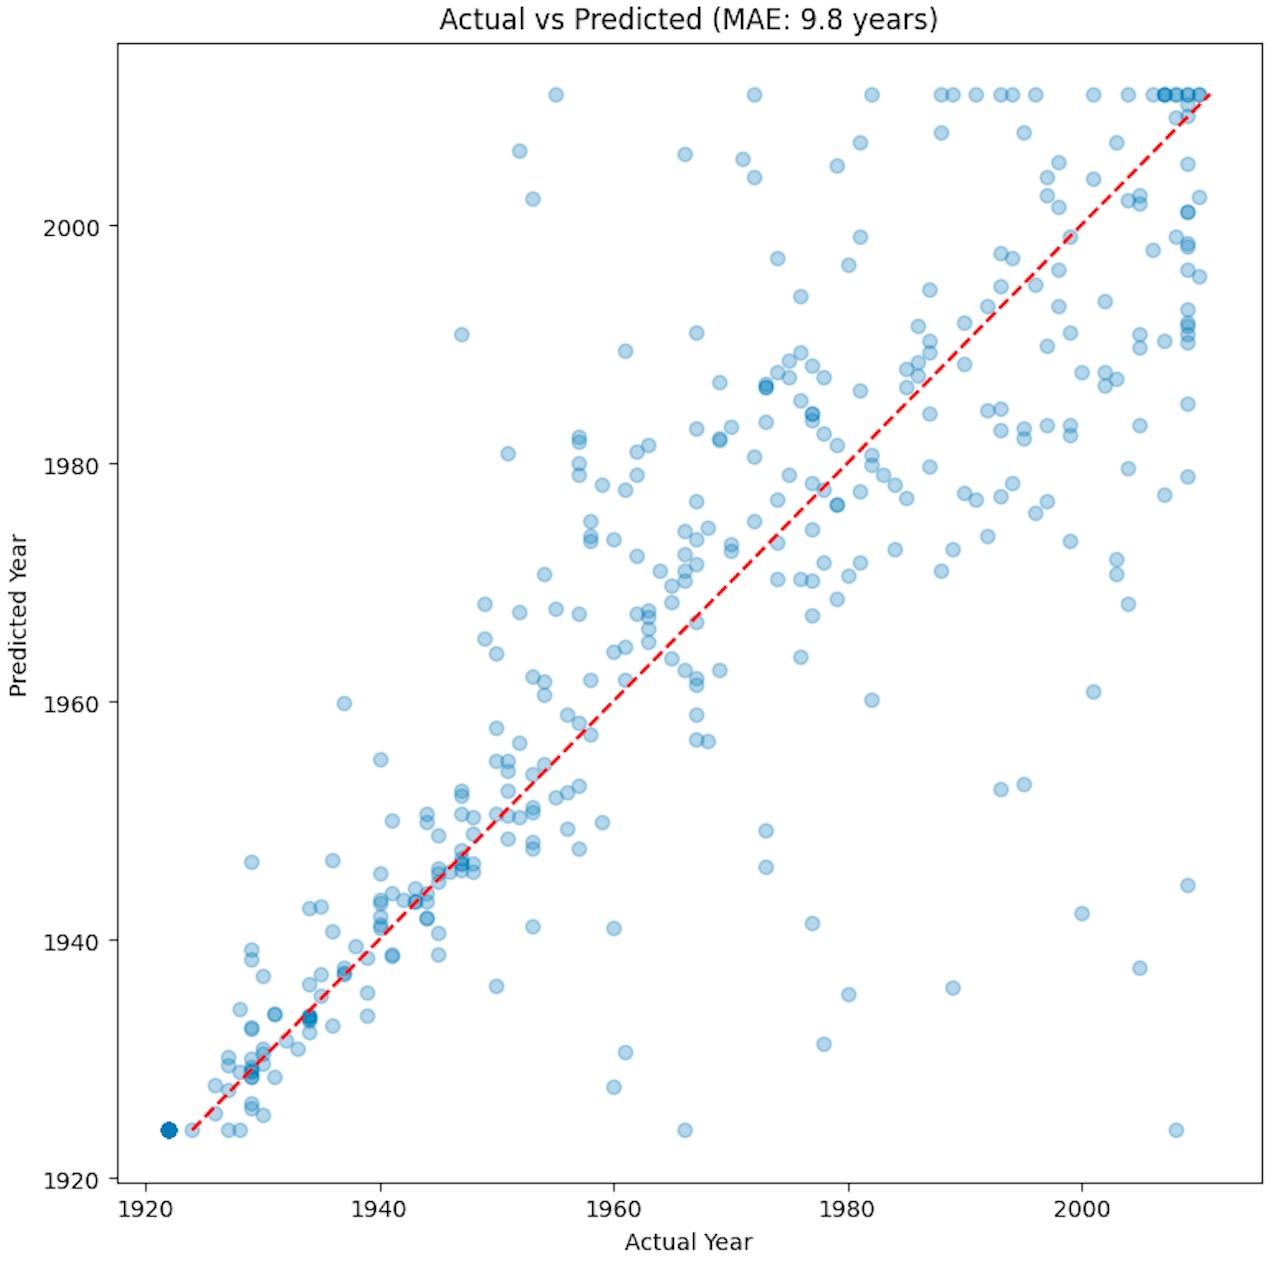
\includegraphics[width=0.5\linewidth]{img/Linear.jpg}
        \end{figure}
        \begin{figure}
            \centering
            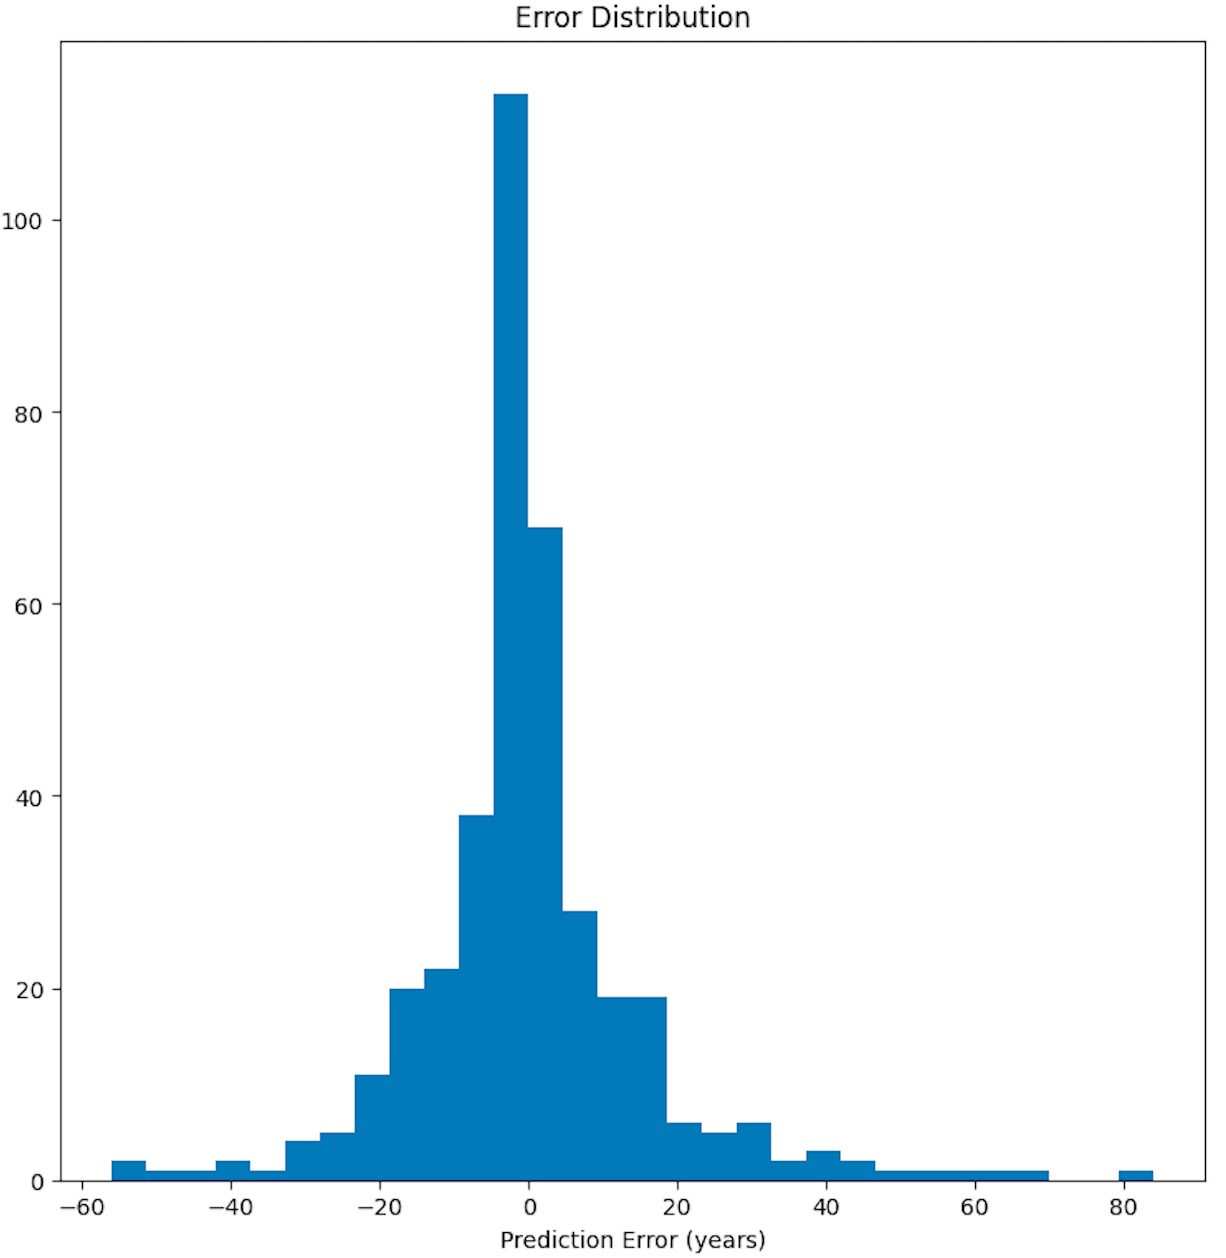
\includegraphics[width=0.5\linewidth]{img/error.jpg}
        \end{figure}
        
	\end{basebox}
\end{textblock}

\begin{textblock}{28.5}(2,65)
	\begin{basebox}[
        decadebox,
        title=Results of Linear Regression with different Principal Components ($k$),
        halign title=right
    ]
    \item \textbf{R\textsuperscript{2}} dropped: 0.26($k=52$) $\rightarrow$ 0.21($k=32$) $\rightarrow$ 0.14($k=10$) \\
	\item \textbf{RMSE} increased: 9.37 $\rightarrow$ 9.73 $\rightarrow$ 10.14 \\
    \item \textbf{SGD Result $k=32$}: R\textsuperscript{2} ~0.21 $\rightarrow$ indicates reached limitations of LR
	\end{basebox}
\end{textblock}

%
% extra content (logos, dev comments, acknowledgements, etc.)
%

\begin{textblock}{16}[1,0](100,0)
	\logos[dark]\qquad
\includegraphics[height=4cm]{img/ece472.pdf}
\end{textblock}

% \begin{textblock}{80}[1,1](100,100)
% 	\begin{tcbraster}[raster equal height,raster column skip=1cm,raster columns=2,raster rows=2, raster row skip=1cm]
% 	\begin{blankbox}[fontupper=\huge,colupper=black]
% 		\authori[Kantaphat Leelakunwet, Choo Lee Wen, Arsen Aghayan, Ibrahim Daurenov]{}
% 	\end{blankbox}
% 	% \begin{blankbox}[fontupper=\huge,colupper=black]
% 	% 	\authori[My comment]{Second author}
% 	% \end{blankbox}
% 	% \begin{blankbox}[fontupper=\huge,colupper=black]
% 	% 	\authori[My comment]{Third author}
% 	% \end{blankbox}
% 	\end{tcbraster}
% \end{textblock}

% \begin{textblock}{45}[0,1](0,100)
% 	\begin{blankbox}[fontupper=\huge,colupper=Black]
% 		Developed in Scala, Powered by Gitea, and Engineered by Team Name
% 	\end{blankbox}
% \end{textblock}

\begin{textblock}{48}[1,1](100,100)
    \begin{blankbox}[fontupper=\huge,colupper=black]
        Kantaphat Leelakunwet, Choo Lee Wen, Arsen Aghayan, Ibrahim Daurenov
    \end{blankbox}
\end{textblock}

\end{frame}

\end{document}
